
\documentclass[11pt, a4paper, USenglish]{article} % change ``USenglish'' to ``norsk'' if applicable.
%\documentclass[10pt,fleqn,oneside]{article}


\usepackage{kyblab} % Contains all included packages. See kyblab.sty.
\usepackage[a4paper, total={460pt, 690pt},hcentering, bindingoffset=0mm]{geometry}

\addbibresource{riktig.bib} % Makes the bibliography file available to biblatex.

%\setcounter{section}{-3}

\usepackage{amsmath}
\usepackage{graphicx}% http://ctan.org/pkg/graphicx
\usepackage{yhmath}% http://ctan.org/pkg/yhmath
\usepackage{mathdots}% http://ctan.org/pkg/mathdots
\usepackage{MnSymbol}% http://ctan.org/pkg/mnsymbol
\usepackage[toc,page]{appendix}
\usepackage{dirtytalk}
\bibliography{riktig}


\begin{document}

% Titlepage
\title{TTK23 Design og analyse for funksjonell sikkerhet}
\author{Kompendium\\
Hanna Waage Hjelmeland}
\date{March 26, 2021}
\begin{titlepage}
    \maketitle
    \begin{figure}[h]
    \centering
        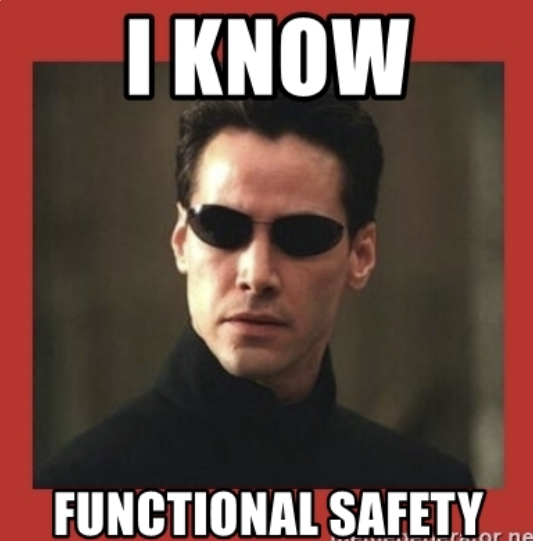
\includegraphics[width=\textwidth]{figures/FaultBasics/robot.png}\\   
    \end{figure}

   \thispagestyle{empty}
\end{titlepage}

% Abstract
%\newpage
%\begin{abstract} 
%\addcontentsline{toc}{section}{Abstract} % add this if you want the abstract in the table of contents.
  This document outlines a few important aspects of a lab report. It contains some advice on both content and layout. The \LaTeX{} source for this document is also published, and you can use it as a template of sorts for your own report. You can find an up to date version of the source at \url{https://github.com/ntnu-itk/labreport}. The main file, ``labreport.tex'', defines the structure of the document. The ``preamble.tex'' file is the document preamble, and contains a lot of informative comments. The document is based on work done by Tor Aksel Heirung for TTK4135, and is now under continuous improvement by Andreas L. Fl{\aa}ten and Kristoffer Gryte (happily accepting suggestions and contributions from the community).

When you write your own report, this section (the abstract) should contain a \emph{very} short summary of what the lab is about and what you have done.
\end{abstract}

%\thispagestyle{empty} % Avoid page numbering on the abstract page.
\newpage
% TOC
\newpage
\tableofcontents
\addtocontents{toc}{\protect\thispagestyle{empty}}
\thispagestyle{empty}
% Avoid page numbering on the table of contents.

% Main content
\newpage
\setcounter{page}{1}
\section{Introduksjon, begreper og IEC 61508}
\label{sec:intro}

\subsection{Funksjonell sikkerhet}

\textbf{Funksjonell sikkerhet dreier seg om sikkerhet som ivaretas av elektriske, elektroniske og programmerbare (E/E/EP) systemer slik at vi kan beskytte mennesker, miljø og infrastruktur fra skade}. Det er et system som utfører en aktiv sikkerhetsfunksjon ved \textbf{behov}, for eksempel et system som henter en båt inn igjen dersom avviket rapportert fra DP-systemet blir for stort. Sikkerhet definerer vi som fravær av uakseptabel risiko.


\subsection{Akronymer og begreper}

\begin{itemize}
    \item \textbf{SCS}: Safety Critical System
    \item \textbf{SIS}: Safety Instrumented System. System med flere SIF-er
    \item \textbf{SIF}: Safety Instrumented Function. The Safety Instrumented Function is a protection layer whose objective is to achieve or maintain a safe state of the process when a specific dangerous event occurs. The SIF is implemented in the SIS (Safety Instrumented System) which is normally composed of several Safety Functions.
    \item \textbf{SIL}: Safety Integrity Level
    \item \textbf{EUC}: Equipment Under Control
    \item \textbf{PFD}: Probability of Failure on Demand
    \item \textbf{PFH}: Probability of Failure per Hour
    \item \textbf{ALARP}: As low as reasonably possible. Et prinsipp som betyr at risiko alltid må reduseres så mye som praktisk mulig. I en risikovurdering kan det være ett tiltak som er teoretisk mulig for å redusere risiko, men som dessverre vil medføre for store kostnader i forhold til hvor mye risikoen reduseres. Og det kan da være helt greit i følge ALARP-prinsippet å ikke utføre tiltaket. Samtidig er man forpliktet til å utføre tiltak som reduserer risiko også selv om risikoen i utgangspunktet ikke framstår som spesielt alarmerende. Man er forpliktet så lenge kostnadene forbundet med tiltakene er akseptable i forhold til vinningen.
    \item \textbf{Hazard}: Potensiell farekilde forårsaket av at komponenten ikke utfører sin funksjon på en tilfredsstillende måte.
\end{itemize}


\subsection{Systemmodeller og metoder}

Vi sier at et system kan beskrives av fire aspekter. Vi bruker et enkelt gressklippe-eksempel for å illustrere.

\begin{itemize}
    \item \textbf{Systemets komposisjon}: Samlingen av delene og objektene i systemet. F. eks. personen og gressklipperen.
    \item \textbf{Miljøet}: Miljøet som systemet operer i. Det som er definert på utsiden av systemet men som både kan påvirke og bli påvirket av systemet. F. eks. plenen.
    \item \textbf{Systemets struktur}: Relasjonene mellom systementiteter som innehar en rolle i systemet, dvs aktører som har en aktiv rolle og kan ta avgjørelser, ha ansvar for måloppnåelse osv. F. eks. kontrollere, aktuatorer, sensorsystemer. F. eks. Personen som klipper plenen. OBS: En aktør kan være både del av komposisjonen og strukturen.
    \item \textbf{Systemets mekanismer}: Prosessene og funksjonene som gjør at systemet oppfører seg som det gjør. 
\end{itemize}

Disse kan illustreres i et \textit{systemtriangel}, hvor emergent oppførsel $\mu(s)$ oppstår i midten som resultat av samhandling mellom de tre hjørnene, og miljøet på utsiden.

\begin{figure}[H]
    \centering
        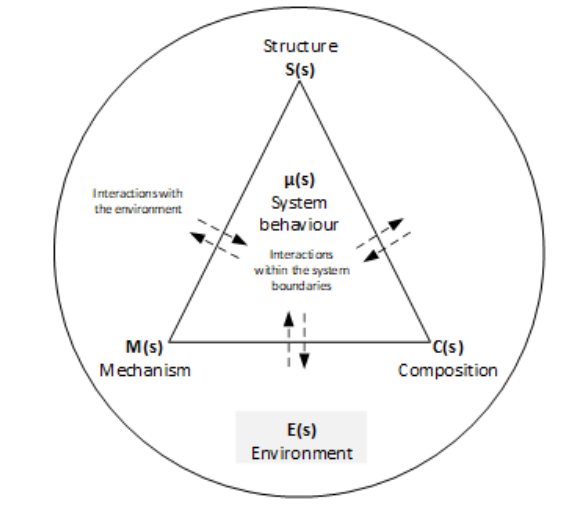
\includegraphics[width=0.7\textwidth]{figures/IEC/cesm.PNG}\\
        \caption{Illustrasjon av de ulike aspektene av CESM-modellen.}
\end{figure}

Aspektene i CESM er både nødvendig og tilstrekkelig for å forstå egenskapene og oppførselen til ethvert system.
For å finne en fullstendig modell av systemet, trenger vi systemmodeller som til sammen adresserer hele CESM metamodellen. Dette kan være vanskelig å få til.  Husk, George Box: Alle modeller er feil;
noen er nyttige, som også betyr at \textbf{ikke alle er nyttige}.

Flere systemmodeller kan representere hver av elementene i CESM. Dette står man fritt til å velge i forhold til
målsetting og situasjon. En "komplett" systemmodell kan dannes med basis i følgende modelltyper som hver for
seg adresserer forskjellige elementer i CESM:


\begin{itemize}
    \item Funksjonsmodell
    \item Aktørmodell
    \item Objektmodell
    \item Målmodell
    \item Modell(er) av oppførsel (emergens $\mu(s)$)
\end{itemize}

\begin{figure}[H]
    \centering
        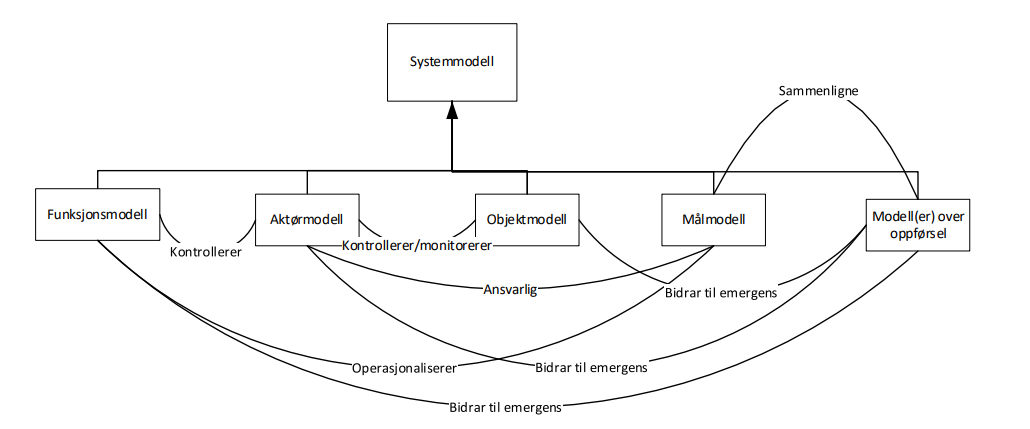
\includegraphics[width=\textwidth]{figures/IEC/systemmodell.PNG}\\
        \caption{Illustrasjon av hvordan de ulike modellene henger sammen, for å beskrive alle elementene i CESM.}
\end{figure}

\subsection{IEC61508}

\textbf{IEC61508} er en internasjonal standard som inneholder krav og analyser for funksjonell sikkerhet.



\subsection{Sikkerhets Livssykel (Safety Lifecycle)}

IEC 61508 definerer livssykelen til et sikkerhetssystem i 16 faser.

\begin{itemize}
    \item[\textbf{1:}] Konsept:  Her defineres EUC og EUC Control System
    \item[\textbf{2:}] Scope definisjon: Avgrensning. Avdekke sentrale krav, operasjonelle antakelser, erfaringer fra tidligere som er nyttig for neste fase.
    \item[\textbf{3:}] Hazard og risiko analyse for EUC og EUC control system. Hazard vil si en farekilde som er en egenskap ved systemet, for eksempel høyt trykk. Først identifiserer man potensielle hazardous events (ofte i en workshop ved hjelp av sjekklister og/eller en strukturert analyse), før man analyserer disse tilfellene i en risikotabell, se tabell under.
    \item[\textbf{4:}] Generelle sikkerhetskrav: Liste sikkerhetskrav av overordnede funksjoner og tiltak som risikoanalysen har avdekket.
    \item[\textbf{5:}] Allokere sikkerhetskrav. Fra risikoanalysen og de risikoreduserende tiltakene får vi formelle krav til sikkerhetssystemet, i tillegg til prioritering og pålitelighetsbehov. 
    
    \textbf{1} - Bestemme hvilke systemer som skal utføre hvilke funksjoner. Skal det være organisatoriske tiltak, menneskelige aksjoner eller aksjoner utført av tekniske systemer som SIS? Og for SIS: Skal funksjonene plasseres i samme SIS, eller i flere SIS?
    
    \textbf{2} - Bestemme pålitelighetskrav til funksjoner som skal utføres av SIS(er) og tilhørende SIL-krav. Pålitelighetskrav kan for eksempel være en gitt PFD og/eller PFH, altså en gitt sannsynlighet for feil og/eller forventet hyppighet av feilen. Merk: Pålitelighetsmålet PFD brukes for SIFer som er low-demand (behov for disse sjeldnere enn en gang i året), mens PFH (frekvens av farlige feil per time) benyttes som pålitelighetsmål for SIFer som er «high-demand/ «continous demand», det vl si hhv behov for oftere enn en gang i året eller kontinuerlig. Vi spør oss altså: Hvor sannsynlig er feilen, eller hvor ofte kan den oppstå?
    
    \item[\textbf{6-8:}] ...
    \item[\textbf{9-10:}] Designe SIS og SIF-er i henhold til SIL krav. Hvor pålitelige skal de være? Hvor skal sikkerhetsfunksjonen plasseres?
    \item[\textbf{11-16:}] ...

\end{itemize}

\begin{table}[]
\begin{tabular}{|l|l|l|l|l|l|l|}
\hline
\begin{tabular}[c]{@{}l@{}}Farlig\\ hendelse\end{tabular}                                                                        & Årsak(er)                                                                                  & \begin{tabular}[c]{@{}l@{}}Worst\\ case\\ konsekvens\end{tabular}                                  & \begin{tabular}[c]{@{}l@{}}Alvorlighet\\ Farlig\\ Hendelse\end{tabular}          & \begin{tabular}[c]{@{}l@{}}Alvorlighet\\ Konsekvens\end{tabular}                 & Risiko                                                                                                                                   & \begin{tabular}[c]{@{}l@{}}Risiko-\\ reduserende\\ tiltak\end{tabular}                                  \\ \hline
\begin{tabular}[c]{@{}l@{}}En hendelse\\ som kan\\ lede til\\ ulykke om\\ den ikke\\ forhindres\\ eller\\ begrenses\end{tabular} & \begin{tabular}[c]{@{}l@{}}Farekilder\\ og\\ triggere\\ (initiating\\ events)\end{tabular} & \begin{tabular}[c]{@{}l@{}}Mhp.\\ personskade,\\ miljø\\ eller\\ materielle\\ verdier\end{tabular} & \begin{tabular}[c]{@{}l@{}}Kategori\\ valgt\\ fra risiko-\\ matrise\end{tabular} & \begin{tabular}[c]{@{}l@{}}Kategori\\ valgt\\ fra risiko-\\ matrise\end{tabular} & \begin{tabular}[c]{@{}l@{}}Enten en\\ score, eller\\ eksempelvis\\ høy (uakseptabel)\\ middels (ALARP)\\ lav (neglisjerbar)\end{tabular} & \begin{tabular}[c]{@{}l@{}}Tekniske,\\ organisatoriske,\\ og/eller\\ menneskelige\\ tiltak\end{tabular} \\ \hline
\end{tabular}
\end{table}

Safety lifecycle utviklingsmetoden skiller seg fra andre metoder ved at det er en risikobasert tilnærming for å sille krav. Man får krav til risikoreduserende tiltak og pålitelighetskrav for SIF-er og SIL-krav. Designprosessen og detaljkravene for realisering blir så styrt av SIL-kravet. SIL-kravet må også følges opp i driftsfasen.

Et eksempel på et risikoreduserende tiltak er å introdusere redundans i systemet, med flere av samme komponent og votering.

\subsection{Bowtie-modellen}

Bowtie-modellen kan brukes for å analysere farlige hendelser og for å plassere sikkerhetstiltak. Den kan også brukes for å identifisere hvor det er behov for SIS og SIFer.

\begin{figure}[H]
    \centering
        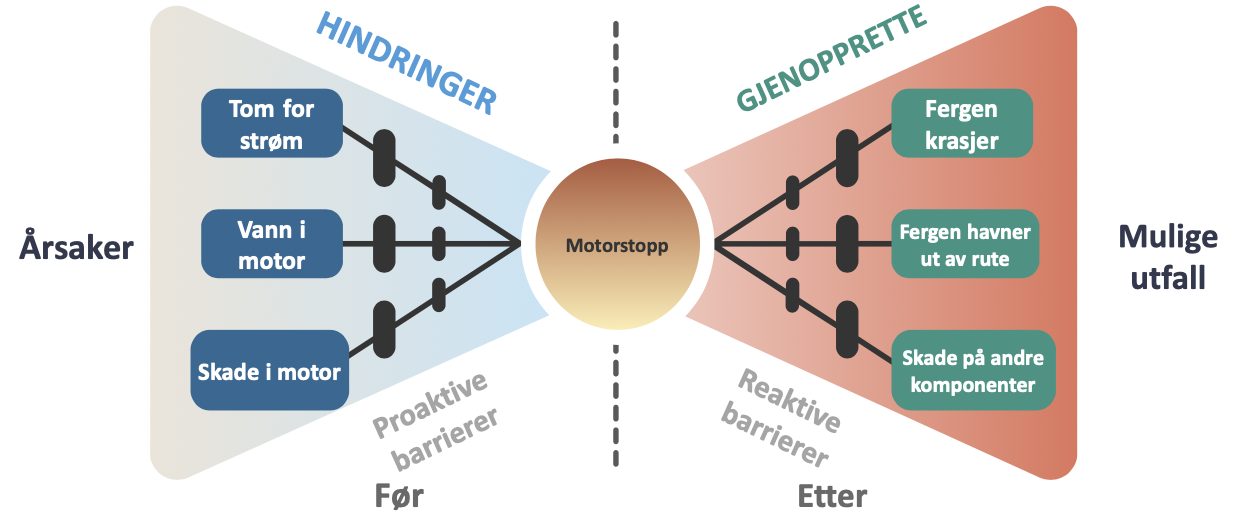
\includegraphics[width=\textwidth]{figures/IEC/bowtie.png}\\
        \caption{Bowtie-analyse for den farlige hendelsen motorstopp.}
\end{figure}

\subsection{SIL-krav}

Et SIL-krav er et krav om at SIF-en vi designer \textit{må} ha PFD og PFH tilsvarende et bestemt SIL-nivå. Høyt SIL-nivå tilsvarer lav sannsynlighet og hyppighet for feil, og vil da indikere en relativt sikker SIF. Lavt SIL-nivå indikerer en mindre sikker komponent og man vil da ofte implementere f. eks. redundans ved votering.
 
For å kunne oppfylle kravene må en ha gjennomført en analyse og klassifisering av de feilene som er registrert på tilsvarende komponenter. For nytt utstyr må en gjøre en analyse (FMEDA – Failure Mode and Diagnosis Analysis) av komponenten for å kunne kvantifisere de forskjellige feilmodiene. Spesielt er det viktig å finne de farlige udetekterte feilene (DU- Dangerous Undetected) som angis med $\lambda_{DU}$ [feil per time].

SIL-kravet får implikasjoner for designet av systemet. Det gir blant annet krav til 

\begin{itemize}
    \item Redundans/votering (per delsystem) ved å stille krav til minimum feiltoleranse.
    \item Krav til diagnostic coverage (evne til å avdekke farlige feil vha diagnostikk: hvor ofte forventer vi å klare å finne feil, og stille riktig diagnose?
    \item Restriksjoner for valg av programmeringsspråk og krav til funksjonalitet i programmeringsverktøy
    \item Krav til at beregnet PFD/PFH for hele SIFen er innenfor SIL-kravet. Dette vil implisitt gi øvre grenser for feilrater for farlige feil, både detekterte og udetekterte, hvor ofte funksjonen testes for å avdekke farlige udetekterte feil, og hvor lang reparasjonstid ifbm farlig detekterte feil.
\end{itemize}

Et eksempel på en SIF og tilhørende SIL-krav:
Fra risikoanalyse og allokering har vi funnet at vi trenger en SIF i form av en av/på-ventil som stenger dersom trykket i tanken blir for høyt. Da trenger vi følgende komponenter:

\begin{itemize}
    \item Sensor
    \item Logisk enhet
    \item Av/på-ventil
\end{itemize}

Fra risikoanalysen ble det funnet at hele SIFen må ha SIL-krav 2. OBS: PFD/PFH skal summeres for alle komponentene som inngår i SIF-en.

\begin{figure}[H]
    \centering
        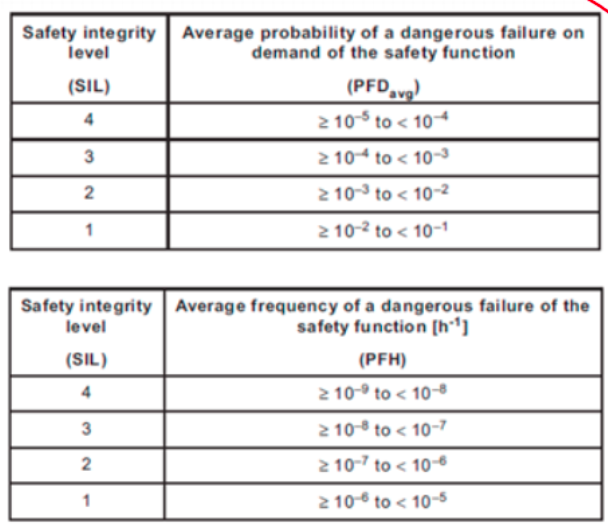
\includegraphics[width=\textwidth]{figures/IEC/sil.png}\\
        \caption{SIL-nivå}
\end{figure}

\subsection{Hvor mye risiko skal vi tillate?}

\begin{figure}[H]
    \centering
        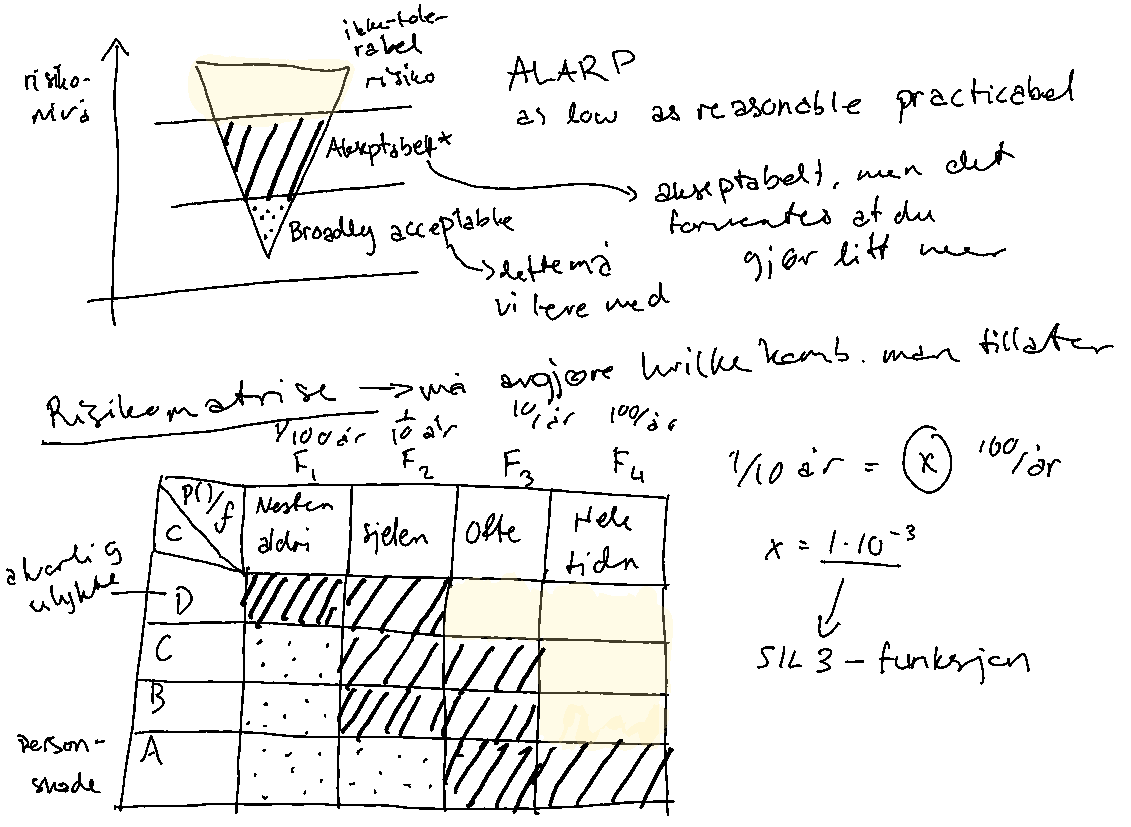
\includegraphics[width=\textwidth]{figures/IEC/risikomatrise.png}\\
        \caption{Risikonivå og risikomatrise. C er farekategori for konsekvens av den farlige hendelsen.}
\end{figure}

\section{Funksjonsanalyse: FAST}
\label{sec:fast}

\subsection{FAST - intro}

FAST står for Function Analisys System Technique, og er en funksjonsanalyse som kan inngå som en del av en systemanalyse. Ved å bruke FAST får vi fram sammenhengen mellom funksjoner, og vi ser hvilke som er avhengig av hverandre. FAST kan også brukes for å samle et team om en idé og sørge for at alle er på samme banehalvdel.


Det mest sentrale konseptet i FAST-teknikken er hvorfor/hvordan-spørsmålet. Ved å stille dette spørsmålet til funksjonene vi har listet opp, får vi kausal-oversikt i systemet.

FAST-teknikken kommer fra feltet Value Engineering, som handler om å skape samme funksjon for mindre kostnad. Dette egner FAST seg spesielt for ettersom metoden identifiserer funksjoner og sammenhenger som gjør det lett å bytte ut funksjoner for å oppnå samme mål.


\subsection{Metode}

FAST gjøres best i team. For å sette i gang kreativiteten, gjør man gjerne en systemdekomponering og lister opp komponentenes funksjoner, før man går videre og setter disse opp i et "hvorfor/hvordan"-diagram. Deretter kan man sette disse sammen i et fullstendig FAST-diagram.

\textbf{Funksjonens navn}: Funksjonens navn spiller en viktig rolle i FAST og det er fafstsatte konvensjoner for hvordan man skal navngi funksjoner. Dette er for å sikre at man er spesifikk nok, og for å sette i gang kreativiteten.
Fuksjonsnavnet skal umiddelbart si noe om formålet bak funksjonen, uten å nødvendigvis si noe om metoden for å gjøre det. Hovedregelen er at funksjoner skal starte med et aktivt verb og avslutte med et substantiv. Eksempler:

\begin{itemize}
    \item Lad batteri
    \item Klipp gress
\end{itemize}

Eksempel på FAST-diagram for ankermekanisme på båt:

\begin{figure}[H]
    \centering
        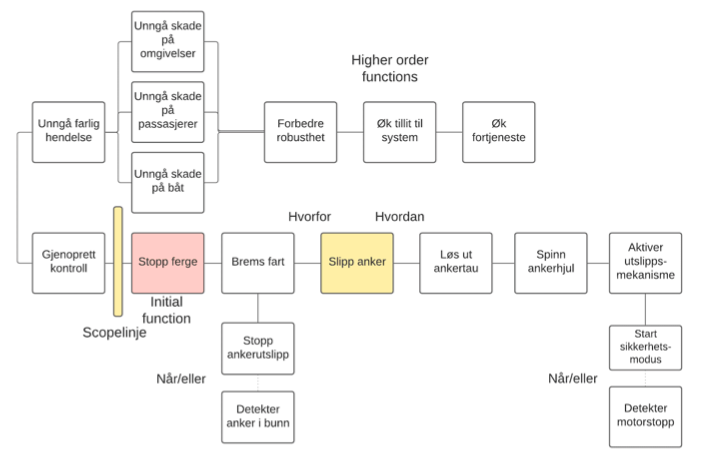
\includegraphics[width=\textwidth]{figures/FAST/Skjermbilde 2021-11-24 kl. 09.28.51.png}\\
        \caption{FAST-diagram for ankermekanisme på båt.}
\end{figure}

Vi ser at i dette FAST-diagrammet er det også gjort litt videre analyse enn bare hvorfor/hvordan. Her er det også lagt inn en såkalt "scopelinje", som er en linje som markerer primærbehovet for mekanismen, det vil si hovedoppgaven til systemet. Scopelinjen settes der hvor man kan si at "dersom funksjonen til høyre for linjen ikke hadde vært der, hadde vi ikke hatt behov for noen av de andre funksjonene heller", også kalt "initial function". I dette tilfellet kan vi se at dette er "Stopp Ferge", som blir hovegrunnen til at vi lnsker å implementere ankermekanismen. Dersom vi ikke ønsket å stoppe fergen, hadde vi f. eks. heller ikke trengt å bremse farten. Funksjonene etter scopelinjen kalles "higher order functions", fordi de ikke er like sentrale for systemet.

Hovedstien i diagrammet kalles "kritisk sti", mens funksjonene som spinner ut derfra kalles sekundærsti.

Vi kan også notere oss at jo lenger til venstre vi kommer i diagrammet, desto mer øker muligheten for innovasjon. Funksjonen "Løs ut ankertau" er en spesifikk funksjon som ikke kan utføres på så mange forskjelllige måter, mens "Stopp ferge" er en funksjon som potenstielt kan ha flere løsninger. Kanskje et automatisk DP-system kan erstatte hele ankersystemet? Da kan man konstruere et alternativt fast-diagram ut fra "Stopp ferge"-funksjonen.

\subsection{Ulemper / Hva som ikke inkluderes i FAST}

FAST inkluderer ikke tidsmessig informasjon som timing eller sekvenser, eller typen av funksjoneller avhengigheter som input/output, ressurs eller betingelser.

\subsubsection{FAST sin rolle i CESM-modellen}

FAST adresserer mekanismene i CESM og funksjonsmodellen. FAST-diagrammet representerer funksjonene som bokser som henger sammen. FAST er god på å bevege seg mellom abstraskjonsnivå. Men: FAST inneholder ingen konsepter som gjør at man kan analysere funksjonene på et gitt abstraksjonsnivå, og kan dermed ikke brukes alene som analysemetode. \textbf{FAST utgjør derimot et godt supplement til STPÅ, siden STPA mangler systematikk for å bevege seg mellom abstraksjonsnivå}. Dermed utfyller de hverandre slik at man gjennom disse to metodene kan adressere CESM på flere abstraksjonsnivå. 
\section{Feil og feilanalyse: FMECA}
\label{sec:fmeca}


\subsection{FMECA intro}

FMECA står for FeilMode Effekt (C)Konsekvens/kritikalitet Analyse og er en metodikk for å analysere feilmoder. Det er en systematisk og strukturert metode med fast oppsett, hvor resultatet presenteres i en FMECA-tabell, se eksempel i figur \ref{fig:fmeca_propell}.

\begin{figure}[H]
    \centering
        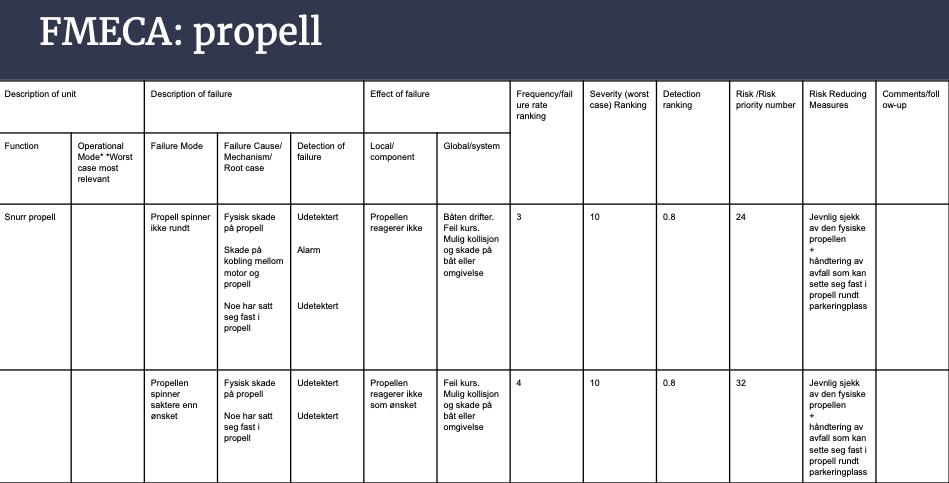
\includegraphics[width=\textwidth]{figures/FMECA/Skjermbilde 2021-11-24 kl. 09.54.55.png}\\
        \caption{Eksempel på FMECA-tabell for propell på båt.}
        \label{fig:fmeca_propell}
\end{figure}

FMECA brukes til å identifisere alle potensielle feilmoder av forskjellige deler av et system, konsekvensene av disse feilmodene, og hvordan vi kan unngå eller minske effekten av feilene.

FMECA er en teknikk for å identifisere, prioritere og eliminere potensielle feil fra et system, design eller prosess før de når kunden.


Ved hjelp av FMECA kan vi få et anslag av systemets \textbf{diagnostic coverage}, det vil si, hvor effektiv vi oppfatter feil i systemet. Matematisk er dette en ratio gitt av forholdet mellom antall detekterte feil, over totalt antall mulige feil.


\subsection{Bakgrunn}
\begin{itemize}
    \item FMECA er en av de tidligste formene for feilanalyse, og ble utviklet av det amerikanske militære.
    \item FMECA blir mest brukt i reliabilitetsanalyse i tidlig stadie i produkt/system-utvikling, vanligvis under konsept- og tidlig design-fase for å sikre at alle potensielle feilmoder har blitt evaluert og at man har på plass riktige tiltak for å eliminere disse feilene.
\end{itemize}

\subsection{Metode}

\textbf{I forkant av FMECA-prosedyren}

\begin{itemize}
    \item[\textbf{1:}] Definer systemet som skal analyseres.
    \begin{itemize}
        \item Systemgrenser (hva skal inkluderes og ikke)
        \item Systemets hovedoppgave og funksjon, inkludert funksjonskrav
        \item Operasjonelle og miljømessige tilstander som bør vurderes
    \end{itemize}
    \item[\textbf{2:}] Samle tilgjengelig informasjon som beskriver systemet som skal analyseres, feks. tegninger, spesifikajsoner, skjemaer ...
    \item[\textbf{3:}] Samle informasjon om tidligere og liknende design fra interne kilder, som intervjuer med designere, vedlikeholdspersonell, osv.
\end{itemize}

\textbf{FMECA-prosedyren}

\begin{itemize}
    \item[\textbf{1:}] Systemdekomponering: Del opp systemet i komponenter, gjerne funksjonelle elementer. Se eksempel i figur \ref{fig:decomp}. Systemdekomponering bør alltid gjennomføres på et høyt nivå, for så å gå i detaljer der hvor uakseptable konsekvenser finnes. 
    \item[\textbf{2:}] FMECA tabell: Hver komponent fra systemdekomponeringen skal analyseres. Alle funksjoner komponenten utøver skal inkluderes, fra alle operasjonsmodene. Deretter spør vi om komponentens feil kan føre til uakseptabel effekt på systemet. Hvis svaret er ja, må komponenten undersøkes videre. I en FMECA-tabell har vi følgende kolonner:
    \begin{itemize}
        \item \textbf{Unik referanse til element}: Eks ID eller tag nummer.
        \item \textbf{Funksjon}: Komponentens funksjoner listes opp. Viktig å liste alle funksjoner. 
        \item \textbf{Operasjonsmoder}: De forskjellige operasjonsmodene for komponenten listes. Eks: Idle, standby, running. Kan utelukkes om operasjonsmoder ikke er relevant.
        \item \textbf{Potensielle feilmoder}: Identifiser alle potensielle feilmoder for hver funksjon og operasjonsmode. En feilmode bør være en form av ikke-suksess for funksjonen. 
        \item \textbf{Årsaker}: Potensielle årsaker til alle potensielle feilmoder listes, eks korrosjon, slitasje.
        IEC61508 skiller på feilårsaker:
        \begin{itemize}
            \item Tilfeildige feil: Feil som kommer tilbake. Eks. Random hardware feil, slitasje, korrosjon. For å handles med tilfeldige feil må man introdusere feilrater og regelmessig testing.
            \item Systematiske feil: Feil som er deterministiske, f. eks. programmeringsfeil. DIsse feilene kan i utgangspunktet korrigeres 100\%. 
        \end{itemize}
        \item \textbf{Deteksjon}: Muligheten for deteksjon av de identifiserte feilmodene listes. Eks diagnostisk testing, menneskelig oppfatning. Noen feilmoder kan detekteres, andre kan ikke. IEC61508 skiller på feilmoder:
        \begin{itemize}
            \item Farlig (dangerous): Farlige feil. Disse deles igjen inn i
            \begin{itemize}
                \item Farlig detektert (DD: Dangerous detected)
                \item Farlig udetektert (DU: Dangerous undetected). F. eks: ventil fungerer ikke, men vi kan ikke vite det fordi den ikke er i bruk. Denne typen feilmoder krever diagnosetesting/sikkerhetstesting
            \end{itemize}
            \item Sikre (Safe): En feil som ikke forhindrer sikkerhetsfunksjon.
        \end{itemize}
        \item Operasjonelle og miljømessige tilstander som bør vurderes
    \end{itemize}
    \item \textbf{Lokale konsekvenser}: Effekt av feilmoden på andre komponenter i subsystemet (grenen i systemdekomponeringen).
    \item \textbf{Globale konsekvenser}: Effekt av feilmode på hele systemet. Sikkerhetseffekter, miljømessige effekter, økonomiske effekter, osv.
    \item \textbf{Feilrater}: For hver feilmode listes en feilrate, det vil si, frekvensen man antar at feilen vil oppstå med. Ofte deler man disse feilratene opp i klasser, se figur \ref{fig:feilrate}.
    \item \textbf{Alvorlighet (severity)}: Alvorligheten av feilmoden er den verste potensielle (men realistiske) globale effekten av feilmoden. Se eksempel på klasser for alvorlighet i figur \ref{fig:alvor}.
    \item \textbf{Deteksjonsrangering}: Rangering av sannsynligheten for at feilen vil bli detektert før systemet når kunder/end-user. Vi brukte et tall mellom 0 og 1, hvor 1 tilsvarte lav sannsynlighet for deteksjon, mens 0 tilsvarte veldig høy sannsynlighet for deteksjon og at man raskt kunne ordne opp i feilen. 
    \item \textbf{Risiko prioritetsnummer}: (Risk priority number), = feilrate x alvorlighet x deteksjonsrangering.
    Sier noe om hvor høyt feilmoden bør prioriteres, og gjør at vi kan plassere feilmoden i risikomatrise, som i figur \ref{fig:riskmat}.
    \item \textbf{Risikoreduserende tiltak}: Mulige handlinger som enten kan rette feilen fullstendig, redusere frekvensen eller unngå alvorlige konsekvenser.
\end{itemize}


\begin{figure}[H]
    \centering
        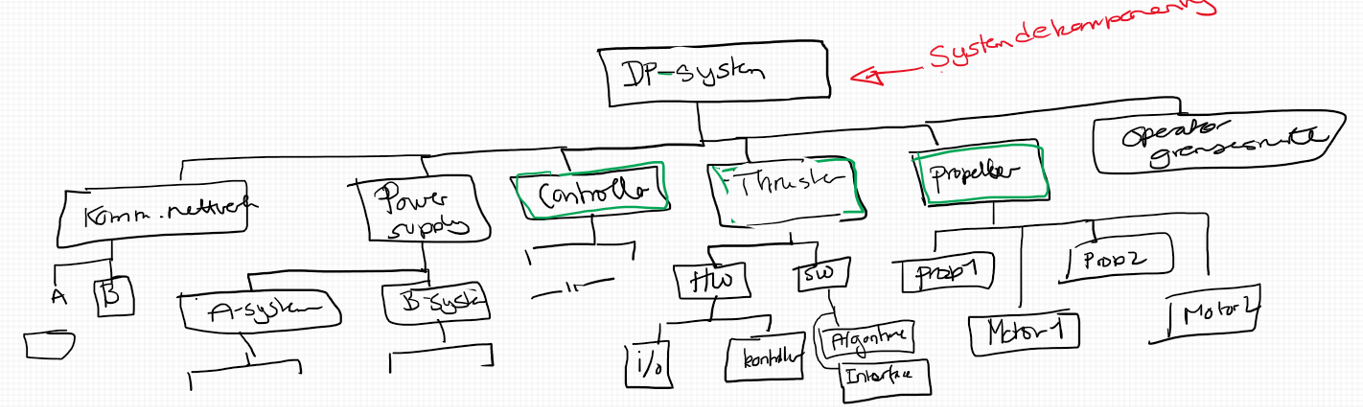
\includegraphics[width=\textwidth]{figures/FMECA/fmeca.PNG}\\
        \caption{Eksempel på systemdekomponering av et DP-system.}
        \label{fig:decomp}
\end{figure}

\begin{figure}[H]
    \centering
        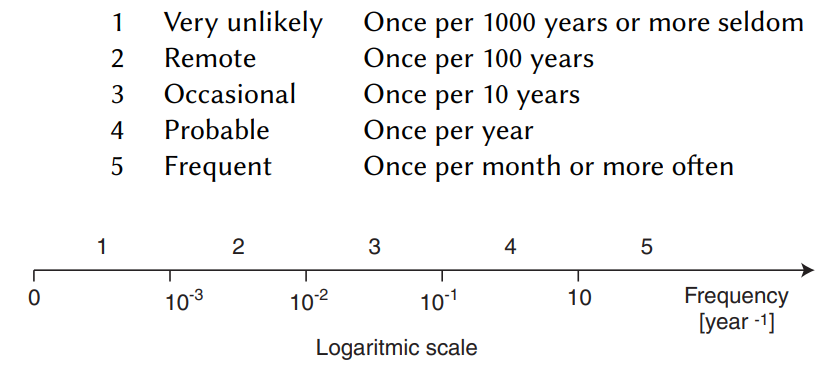
\includegraphics[width=\textwidth]{figures/FMECA/freq.PNG}\\
        \caption{Eksempel på klasser for feilrater.}
        \label{fig:feilrate}
\end{figure}

\begin{figure}[H]
    \centering
        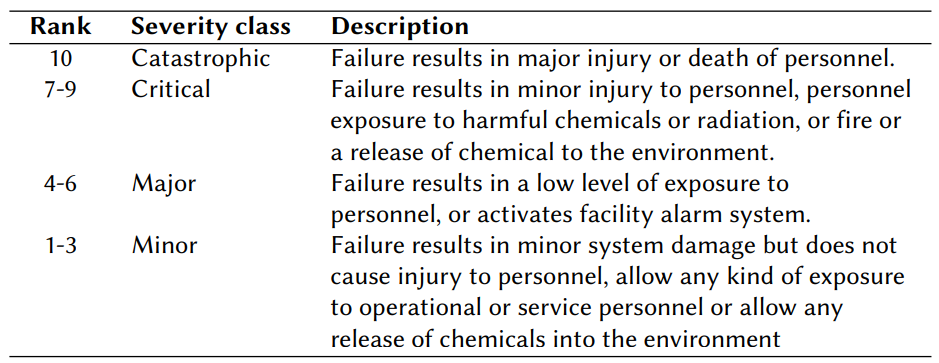
\includegraphics[width=\textwidth]{figures/FMECA/sever.PNG}\\
        \caption{Eksempel på klasser for alvorlighet.}
        \label{fig:alvor}
\end{figure}


\begin{figure}[H]
    \centering
        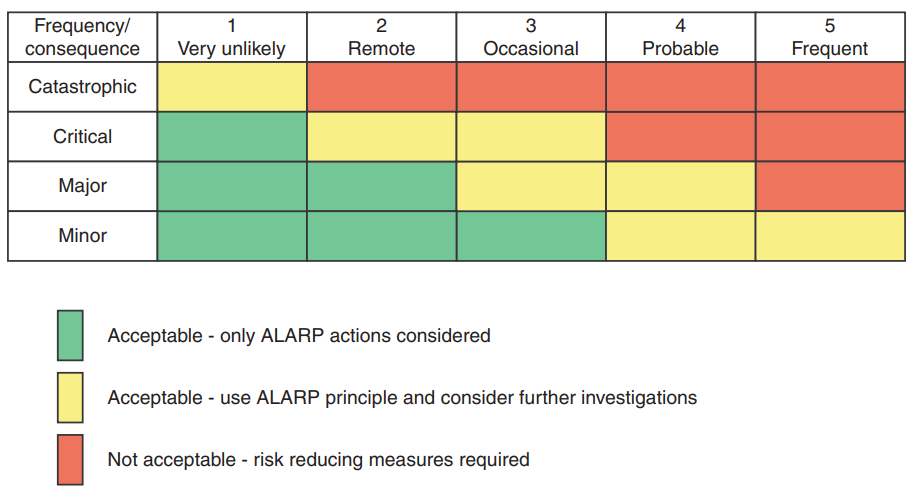
\includegraphics[width=\textwidth]{figures/FMECA/riskmat.PNG}\\
        \caption{Eksempel på risikomatrise brukt i FMECA.}
        \label{fig:riskmat}
\end{figure}

\subsection{Fordeler og ulemper med FMECA}

\textbf{Fordeler}

\begin{itemize}
    \item FMECA er en veldig strukturert og pålitelig metode for å evalurere systemer
    \item Konseptet er enkelt å lære, også for nybegynnere
    \item Tilnærmingen fjør at det er enkelt å analysere også ganske komplekse systemer.
\end{itemize}

\textbf{Ulemper}

\begin{itemize}
    \item FMECA-prosessen kan være kjedelig, tidkrevende og dermed også dyr
    \item Konseptet evaluerer ikke muligheten for flere feil på en gang, noe som ofte er
    tilfellet i praksis.
    \item Det er lett å neglisjere menneskelige feil i analysen.
\end{itemize}
\section{System-Theoretic Process Analysis - STPA}
\label{sec:stpa}

\subsection{Metode}

\begin{figure}[H]
    \centering
        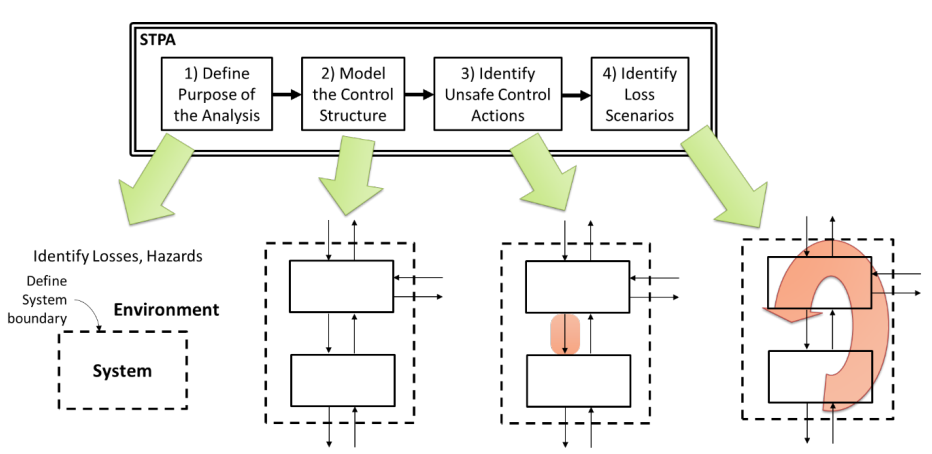
\includegraphics[width=\textwidth]{figures/STPÅ/stpamethod.PNG}\\
        \caption{Oversikt over stegene i STPA-metoden.}
\end{figure}


\subsubsection{Steg 1: Definer formålet med analysen}

I steg 1 skal tap, potensielle hazards og systembegrensninger (constraints) defineres. 
For å definere systemnivå hazards må vi først definere systemet og systemgrensene. Hva skal inkluderes i systemet og ikke?

\begin{itemize}
    \item[\textbf{1}]: Identifiser tap, dvs noe vi potensielt kan miste dersom systemet ikke oppfører seg som ønsket, f. eks. penger, livskvalitet, kundefornøydhet. List dem som "L-1: Tap av liv eller skade på folk, L-2: ...".
    \item[\textbf{2}]: Identifiser system-nivå farekilder (hazards). ISTPA defineres hazard som en systemtilstand som, sammen med et sett av worst-case miljøbetingelser, leder til et tap. List dem, sammen med tapene de potensielt kan føre til "H-1: Båten kommer for nærme andre båter [L-1], H2: ..."
    \item[\textbf{3}]: Definere systemnivå begrenssninger (constraints): Tilstander eller oppførsel som må være oppfylt for å unngå farekilder (hazards), og til slutt forebygge tap. List dem sammen med hazardene de skal unngå, som "SC-1: Båt må opprettholde minimum distanse på 10 m fra andre båter [H-1]".
    \item[\textbf{4}]: Valgfritt: raffinere systemnivå farekilder (hazards): Del hazardsene inn i sub-hazards om ønskelig.
\end{itemize}

Musefelle-eksempel på to runder med dette:

\textbf{Definere systemgrenser}:

\begin{itemize}
    \item \textbf{Objekter}: Musefella, eier av området, åte
    \item \textbf{Aktører}: Musefella og eier av område
    \item \textbf{Mekanismer/funksjoner/Mål:} Drepe mus, Legge på åte, «lade» musefella
    \item \textbf{Miljø} (utenfor vårt system, men som kan påvirke, eller blir påvirket av vårt system):
    \begin{itemize}
        \item Objekter: Hytte, mus, andre dyr, …
        \item Aktører: Mus, andre dyr og fugler (f.eks. rev, ekorn, røyskatt, mink, kråke, ugle), naboen, regelverk, barna, …
        \item Mekanismer: Tiltrukket av åte, Spise åte, Hindre musefellas funksjon, Spise mus, Flytte musefelle, Utløse musefelle,…
    \end{itemize}

\end{itemize}

 Det å ha et bevist forhold til CESM i denne fasen er verdifullt da vi
allerede har indikasjoner på at ikke alt trenger å fungere slik vi hadde tenkt.

\textbf{Runde 1}:

\begin{itemize}
    \item Tap: Tap av livskvalitet 
    \item Hazard: Sykdom [L-1]
    \item Safety-constraint: Unngå smitte
\end{itemize}

\textbf{Runde 2}:

Refined hazard: Smitte fra mus [L-1]. Mer på musefelle-nivå:
\begin{itemize}
    
    \item H-1: Musefelle dreper ikke mus [L-1]
    \item SC-1: Musefelle må lukke seg for å drepe den [H-1]

\end{itemize}

\subsubsection{Steg 2 - Modellere hierarkisk kontrolldiagram}

Et hierarkisk kontrolldiagram er en systemmodell som består av kontroll-tilbakekoblinger. En effektiv kontrollstruktur vil pålegge begrensninger (constraints) på hele systemets oppførsel.

Eksempel:

\begin{figure}[H]
    \centering
        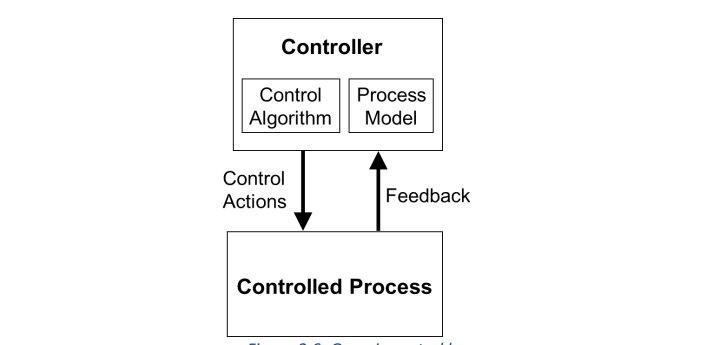
\includegraphics[width=\textwidth]{figures/STPÅ/hier.PNG}\\
        \caption{Generisk kontroll-tilbakekobling.}
\end{figure}

Eksempel fra musefelle-case:

\begin{figure}[H]
    \centering
        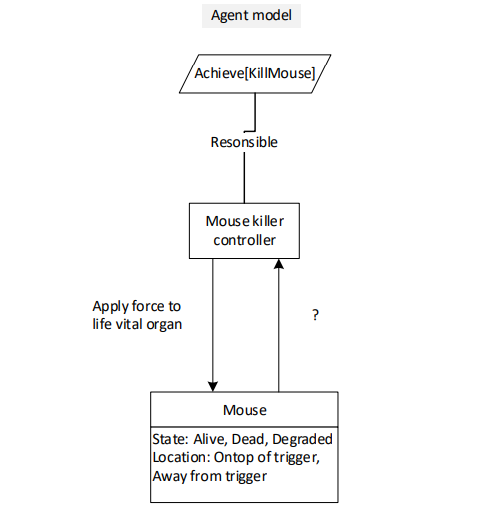
\includegraphics[width=0.5\textwidth]{figures/STPÅ/mus_kontroll.PNG}\\
        \caption{Musefelle-kontrollstruktur.}
\end{figure}

\textbf{Merk}: Kontrollstrukturene kan se veldig annerledes ut, avhengig av hva de skal sette søkelys på. 

\begin{figure}[H]
    \centering
        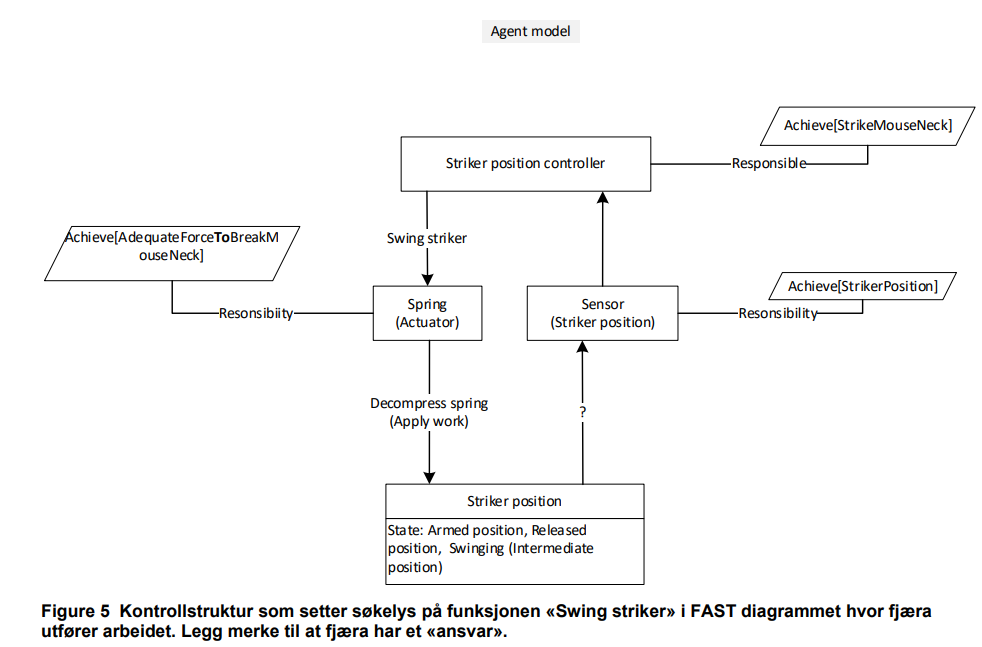
\includegraphics[width=0.5\textwidth]{figures/STPÅ/spring.PNG}\\
        
\end{figure}

\subsubsection{Steg 3 - Identifiser usikre kontrollhandlinger (unsafe control actions)}

Når kontrolldiagrammet er laget, kan vi identifisere usikre kontrollhandlinger. Disse skal listes opp i en tabell og knyttes mod hazardsene som ble definert i steg 1. Eksempel fra STPA-håndbok:


\begin{figure}[H]
    \centering
        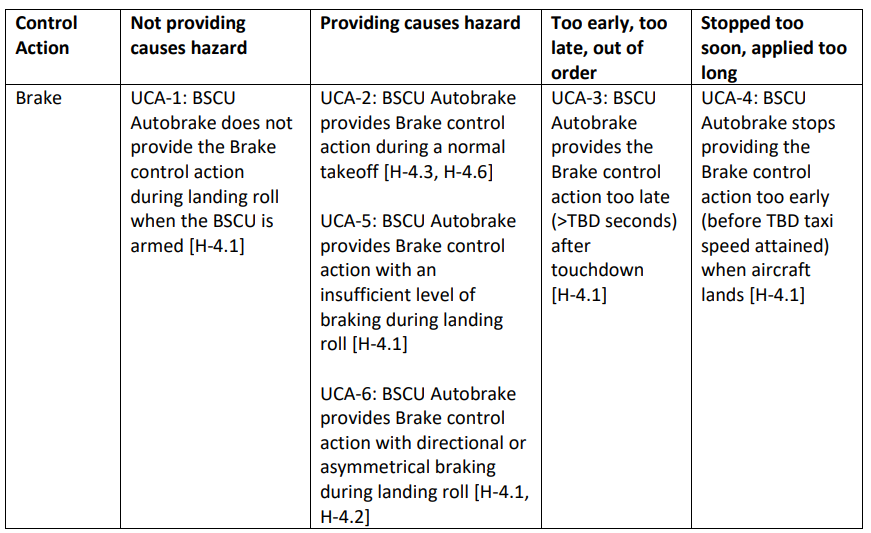
\includegraphics[width=0.8\textwidth]{figures/STPÅ/eks_brake.PNG}\\
        \caption{Eksempel på hvordan man definerer UCAs.}
\end{figure}

Musefelle-eksempel:

\begin{figure}[H]
    \centering
        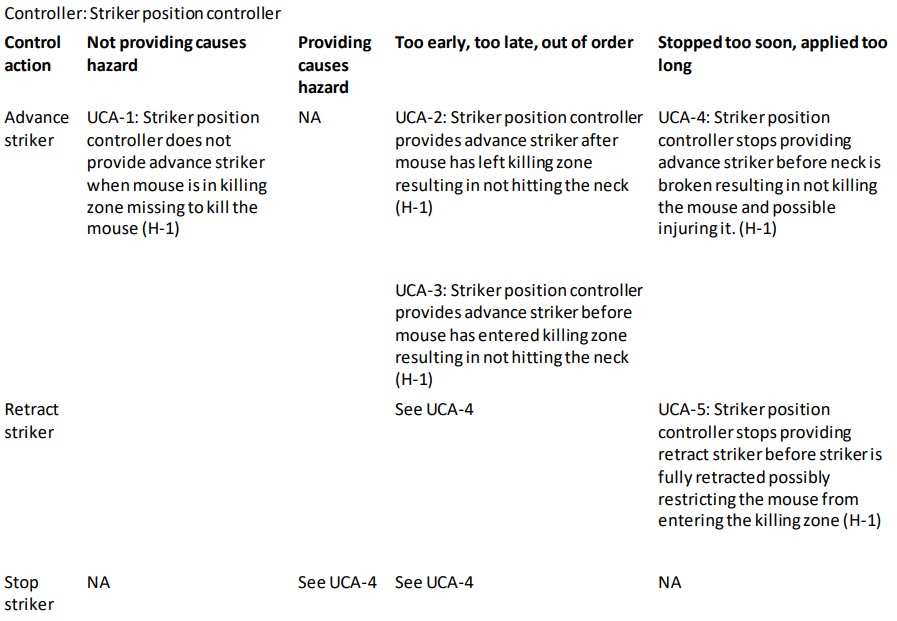
\includegraphics[width=\textwidth]{figures/STPÅ/striker.PNG}\\
        \caption{UCAs i musefelle-eksempel.}
\end{figure}


\textbf{Identifisere safety constraints fra UCAs:}
Når UCA-ene er blitt definert, kan vi oversette disse til begrensninger for systemet som må oppfylles for å forhindre nettopp disse UCA-ene. 

Eksempel fra STPA-håndbok:


\begin{figure}[H]
    \centering
        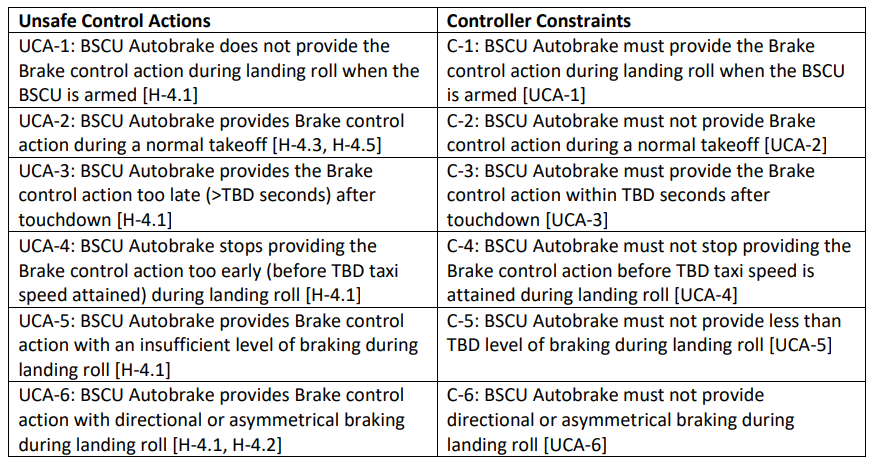
\includegraphics[width=0.9\textwidth]{figures/STPÅ/sc_eks.PNG}\\
        \caption{Eksempel på hvordan man definerer SCs fra UCAs.}
\end{figure}

Eksempel fra musefelle-analyse:

\begin{figure}[H]
    \centering
        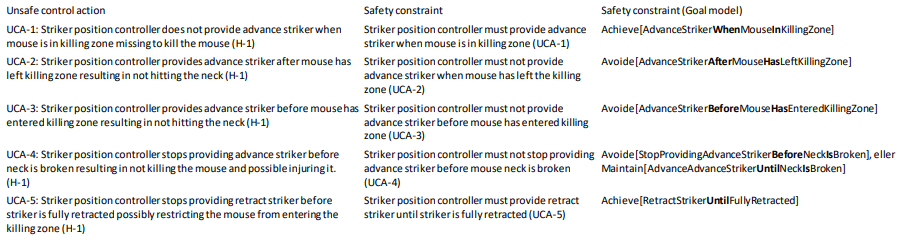
\includegraphics[width=\textwidth]{figures/STPÅ/sc_mus.PNG}\\
        \caption{Eksempel på hvordan man definerer SCs fra UCAs fra musefelle-eksempel.}
\end{figure}

\subsubsection{Steg 4 - identifisere taps-scenarioer}

I steg 4 skal man finne scenarioer hvor UCA-ene kan oppstå, ved å gå rundt kontrollstrukturen for å finne mulige årsaker.

Det gjøres slik, illustrert i håndboken:

\begin{figure}[H]
    \centering
        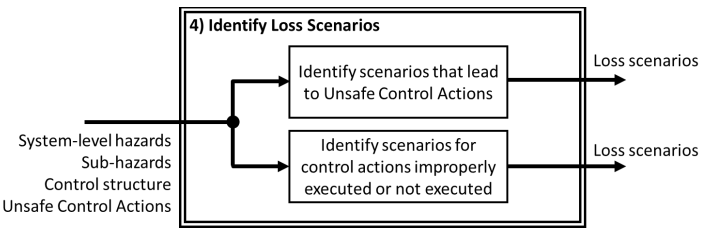
\includegraphics[width=0.9\textwidth]{figures/STPÅ/step4.PNG}\\
        \caption{Steg 4 - definere tapsscenarioer.}
\end{figure}

Eksempel fra musefelle-analyse:

\begin{figure}[H]
    \centering
        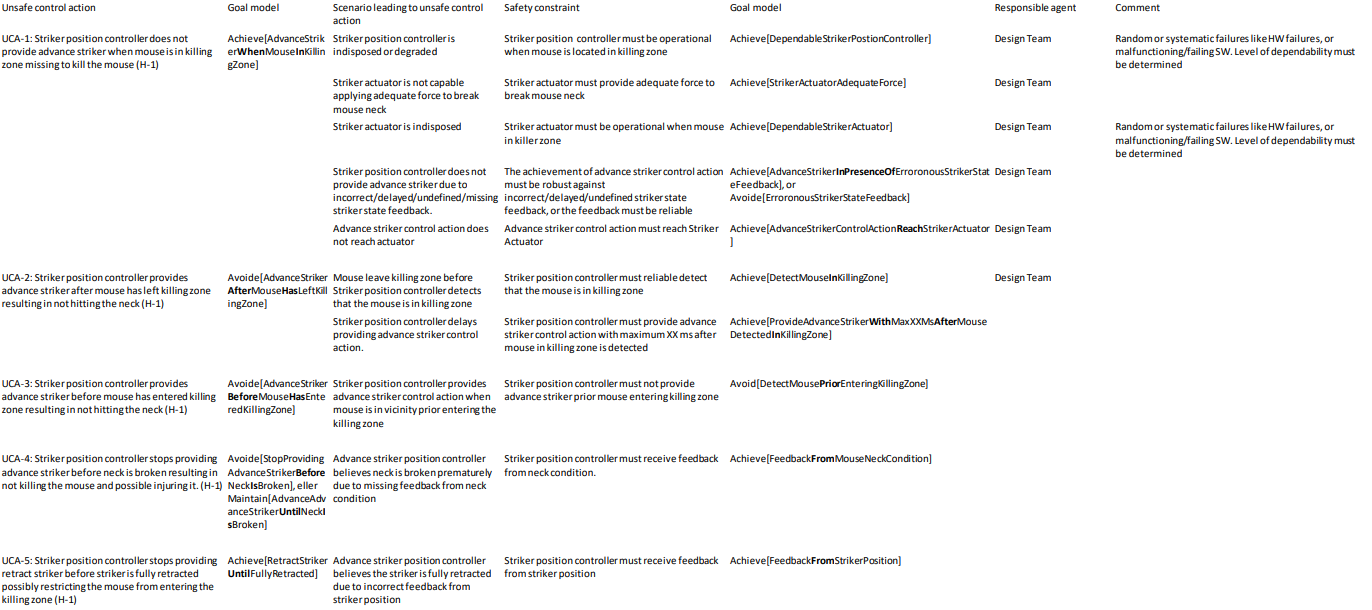
\includegraphics[width=\textwidth]{figures/STPÅ/step4_mus.PNG}\\
        \caption{Tapsscenarioer fra musefelle-eksempel.}
\end{figure}


\subsection{STPA sin rolle i CESM}

Det hierarkiske kontrolldiagrammet inneholder kontroller og den kontrollerte prosesse. Kontrolleren representerer aktøren i strukturen i CESM, dermed er det en aktørmodell. Men dette er bare utgangspunktet, og metoden adresserer de fleste av de andre modellene. En aksjon kan sies å være en funksjon som utføres av en aktør, dermed adressserer control action funksjonsmodellen (mekanismer i CESM). Videre skal man finne scenarioer for hvordan "Unsafe control actions" kan lede til fare definert i første steg gjennom såkalte guidewords. Deretter skal man undrsøke kontrollstrukturen for å finne scenarioer for hvordan sikkerhetsbegrensningene kan bli brutt. Dermed addresseres også målmodellen og modell for oppførsel av systemet, eller ev, hvordan man ikke vil at systemet skal oppføre seg. 

\begin{figure}[H]
    \centering
        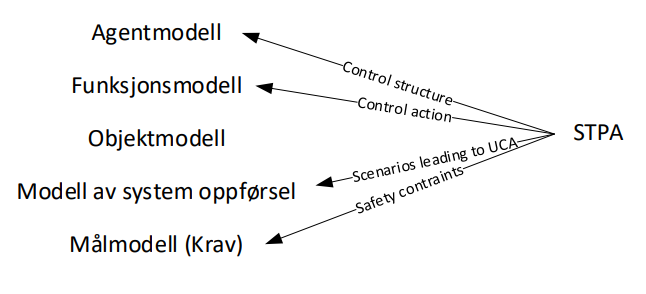
\includegraphics[width=0.7\textwidth]{figures/STPÅ/stpa_cesm.PNG}\\
        \caption{Hvordan de ullike delene av STPA relaterer til CESM-metamodellen.}
\end{figure}


\subsection{STPA vs FMECA}

STPA er konkurrerende med FMECA i å være en større og grundigere analyse av systemet. De leverer ofte liknende resultater. 

I STPA idenfiseres flere nyanser av feil. Dette fordi man, i analysen av UCA-ene, blir tvunget til å analysere funksjonene under spesifikke omstendigheter, eks "Providing causes hazard". Eksempel fra analyse av thrusterkontroller:

\begin{itemize}
    \item \textbf{Feilmoder FMECA}:
    \begin{itemize}
        \item Ingen pådragsreferanse
        \item Feil pådragsreferanse
    \end{itemize}
    \item \textbf{UCAs fra STPA}:
    \begin{itemize}
        \item Manglende pådragsreferanse
        \item Feil pådragsreferanse
        \item Sepunkt settes ved feil tidspunkt
        \item Setpunkt fjernes for fort
        \item Setpunkt holdes for lenge
    \end{itemize}
\end{itemize}

I tillegg er perspektivet på samhandling litt annerledes i de forskjellige metodene. I STPA er det "ovenfra og ned", og aktøren over prosessen har "ansvar" for prosessen, og man analyserer hvordan aktøren kan feile i sin kontroll. 


Vi ser også at i STPA har vi et predefinert sett med tap som UCAsene og hazardsene knyttes opp mot. I FMECA defineres effektene av feilene litt "on-the-go". SLik får man illustrert sammenhenger mellom aktører, funksjoner og konsekvenser i STPA, hvor dette ikke kommer like godt fram i FMECA.


\textbf{MERK}: FAST er ikke en konkurrerende analysemetode, men kan fungere som et godt supplement til begge metodene.

\section{AI sikkerhet}
\label{sec:ai}

\subsection{Hvordan kan bruk av AI påvirke sikkerhetssystemer?}

\begin{itemize}
    \item Måten man innhenter treningsdata for maskinlæringsmodellen har mye å si for resultatet.
    \item Selv om maskinlæringsmodellen er god og har vist bra resultater på andre områder, vil den ikke være bedre enn treningsdataen man henter inn.
    \item Feil eller biased treningsdata kan gi helt feil bilde på situajsonen. Vi så f. eks. at GP-modellen rapporterer lav usikkerhet med OAT-sampling, selv om modellen var helt feil. Dermed kan det også være mye usikkerhet i modellens egen evne til å vurdere usikkerhet, og der kan det oppstå problemer.
    \item Hvis vi i utgangspunktet har høy tillit til ML-modellen kan dette føre til at vi stoler blindt på resultatet, og glemmer å dobbeltsjekke.
    \item Et feil bilde av situasjon/miljø/problem kan gi store konsekvenser og i verste fall føre til svikt/skade på systemet.
\end{itemize}


\subsection{Hvordan kan vi oppdage feil eller redusere konsekvenser??}

\begin{itemize}
    \item Måten man innhenter treningsdata for maskinlæringsmodellen har mye å si for resultatet.
    \item Selv om maskinlæringsmodellen er god og har vist bra resultater på andre områder, vil den ikke være bedre enn treningsdataen man henter inn.
    \item Feil eller biased treningsdata kan gi helt feil bilde på situajsonen. Vi så f. eks. at GP-modellen rapporterer lav usikkerhet med OAT-sampling, selv om modellen var helt feil. Dermed kan det også være mye usikkerhet i modellens egen evne til å vurdere usikkerhet, og der kan det oppstå problemer.
    \item Hvis vi i utgangspunktet har høy tillit til ML-modellen kan dette føre til at vi stoler blindt på resultatet, og glemmer å dobbeltsjekke.
    \item Et feil bilde av situasjon/miljø/problem kan gi store konsekvenser og i verste fall føre til svikt/skade på systemet.
\end{itemize}

\begin{itemize}
    \item Sørge for å ha stort nok sett med treningsdata
    \item Generere kunstige treningsdata for å utvide settet
    \item Bruke adaptive metoder (slik som AL) for å sample oftere der usikkerheten er stor
    \item Bruke ulike sampling- og/eller ML-metoder og vurdere enighet mellom resultatet av disse metodene
    \item Fleksibel nok for komplekse modeller
    \item Begrensninger som gir en modell forståelig for mennesket slik at mennesker kan debugge
    \item Mulighet for menneskelig inngripen i potensielt farlige situasjoner
    \item Få systemet til å reagere på hendelser definert uavhengig av ML-modell
\end{itemize}

\section{Cybersikkerhet}
\label{sec:cyber}


\subsection{PURDUE: Nettverksarkitektur}

PURDUE er en nettverksarkitektur med ulike nettverksnivåer, hvor hvert nivå har et eget nettverk. 

\begin{itemize}
    \item \textbf{Information Technology - del}:
    \begin{itemize}
        \item Nivå 4: Enterprise/kontornettverk
    \end{itemize}
    \item \textbf{Operational technology (styringssystemer) - del}:
    \begin{itemize}
        \item Nivå 3.5: DMZ (demillitarisert)-sone mellom nivå 4 og 3, eks brannmur. Fra wikipedia: En DMZ eller demilitarisert sone i datanettverk er et fysisk eller logisk subnet som offentliggjør en organisasjons offentlige tjenere mot internett. 
        \item Nivå 3: Servere til datainnsamling. 
        \item Nivå 2: Overvåkning (kontrollrom). Eget nettverk med kontrollert forbindelse.
        \item Nivå 1: Kontrollere (SIF-er og basic kontrollenheter)
        \item Nivå 0: Sensorer/prosessutstyr - busser, analoge signaler, IO-utstyr osv.
    \end{itemize}
\end{itemize}


\begin{figure}[H]
    \centering
        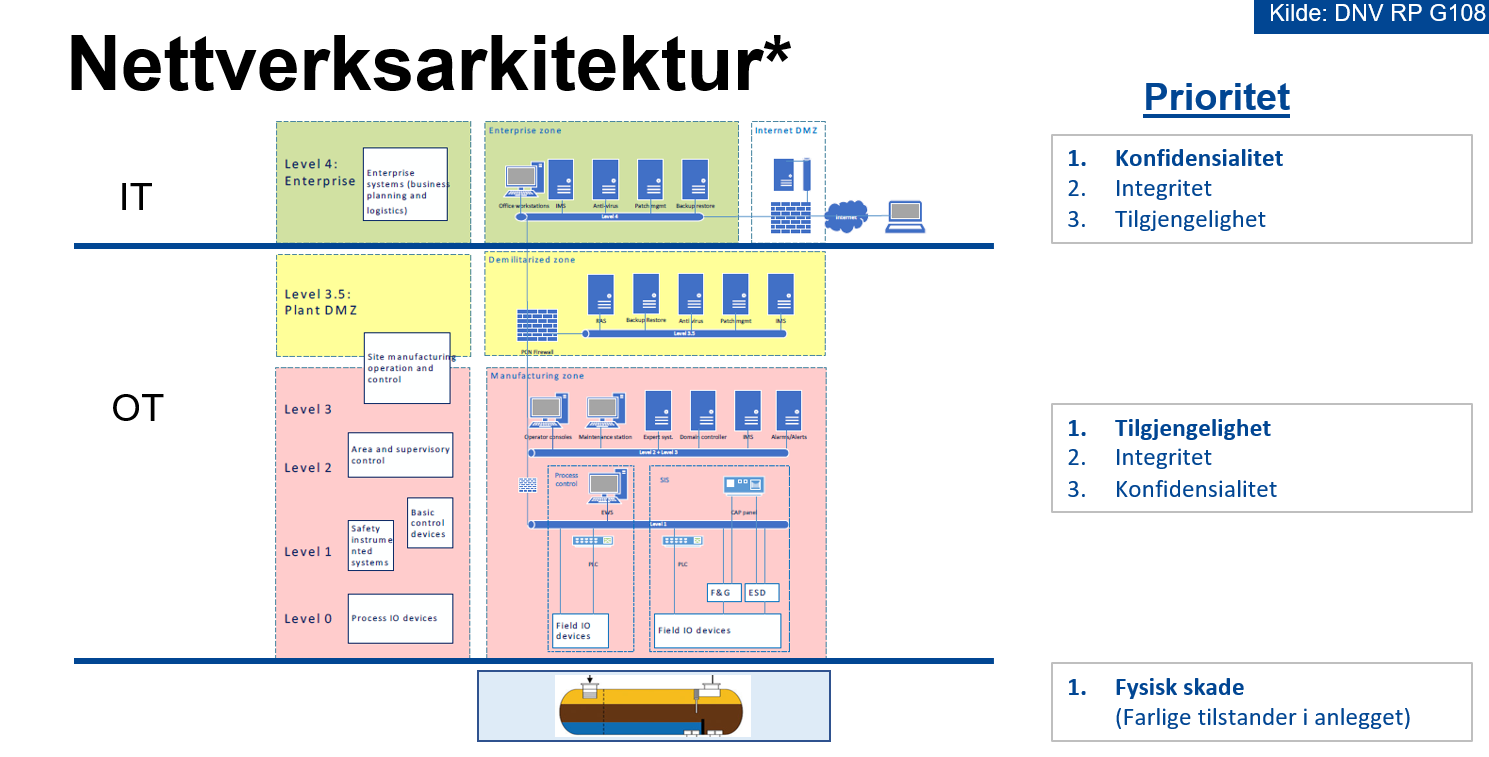
\includegraphics[width=\textwidth]{figures/cyber/purdue.PNG}\\
        \caption{PURDUE referansearkitektur.}
\end{figure}

\subsection{Beskyttelsestiltak}

IEC62443 er bibelen for standarder vedr. industrielle kommunikasjonsnettverk. I standarden defineres SL (security level) -krav, analogi til SIL-kravene, se figur. 

\begin{figure}[H]
    \centering
        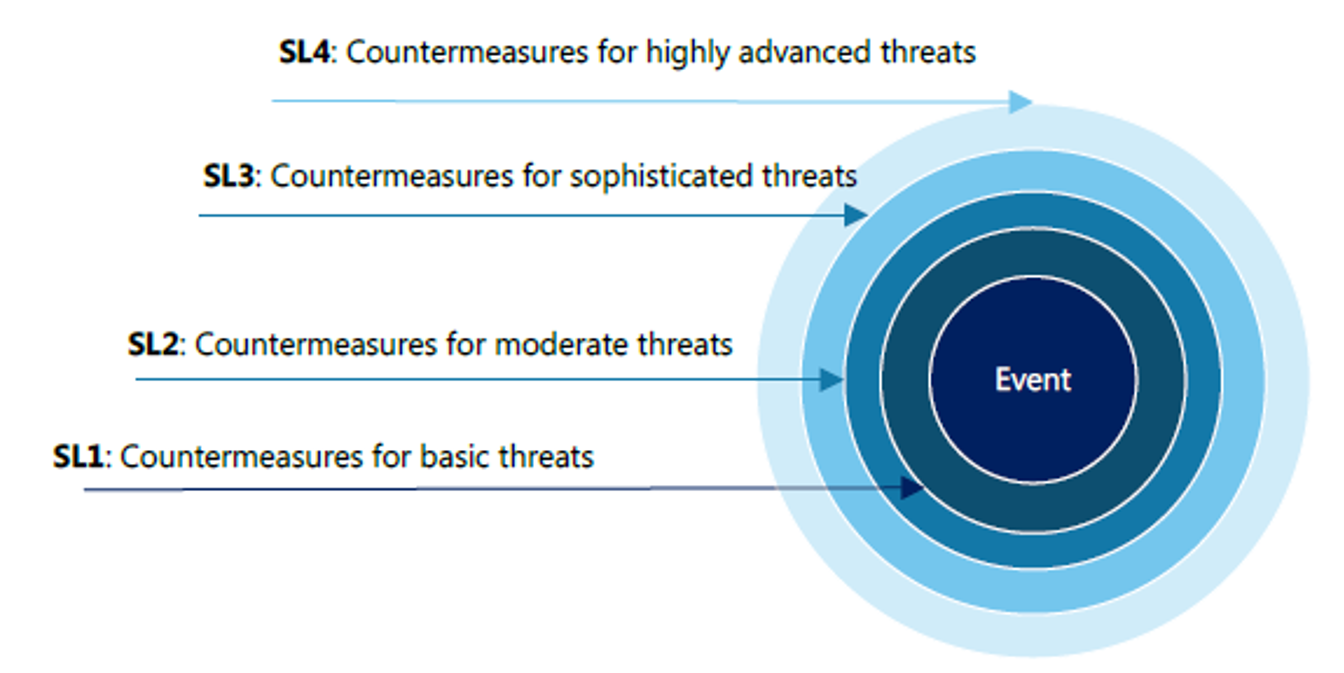
\includegraphics[width=\textwidth]{figures/cyber/sl-krave.PNG}\\
        \caption{De fire nivåene med SL-krav.}
\end{figure}

Standarden beskriver steg for å bestemme soneinndeling, tuneller mellom sonene, og SL-krav til sonene. Tommelfingerregler:

\begin{figure}[H]
    \centering
        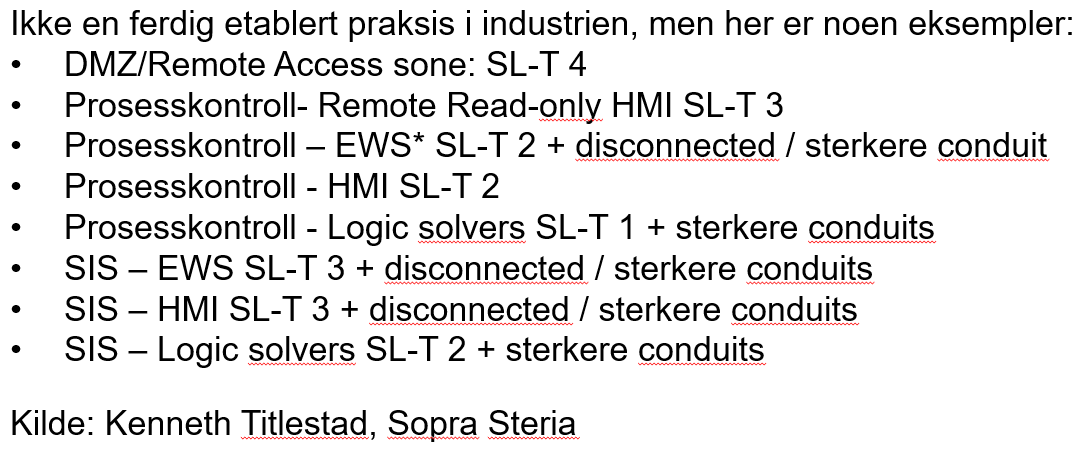
\includegraphics[width=\textwidth]{figures/cyber/tommel.PNG}\\
        \caption{Tommelfingerregler for SL-krav til soner.}
\end{figure}

IEC identiserer også ulike kategorier for beskyttelsestiltak:

\begin{itemize}
    \item [\textbf{FR 1}] – Identification and authentication control
    \item [\textbf{FR 2}] – Use control
    \item [\textbf{FR 3}] – System integrity 
    \item [\textbf{FR 4}] – Data confidentiality 
    \item [\textbf{FR 5}] – Restricted data flow
    \item [\textbf{FR 6}] – Timely response to events 
    \item [\textbf{FR 7}] – Resource availability
\end{itemize}


\subsection{CYPHASS-metoden}

CYPHASS-metoden er egentlig et komplekst bowtie-diagram som bidrar til å identifisere risiko for at feil forplanter seg fra cyberlaget og videre til det fysiske laget. På veien i analysen kan vi også identifisere deteksjon og sikkerhetsbarrierer for å hindre feilene i å forplante seg videre.
\section{Oppsummering}
\label{sec:oppsum}

\begin{itemize}
    \item FAST er en funksjonanalyse som ser på samhandlingen mellom funksjonene i systemet. FMECA ser på én og en funksjon, og analyserer feilmoder assosiert med den.
\end{itemize}






% \input simply inserts the contents of the file, while \include forces a \newpage.
% See \input vs. \include: http://tex.stackexchange.com/questions/246/when-should-i-use-input-vs-include

% References
\newpage
%\addcontentsline{toc}{section}{References}
\printbibliography
\label{sec:bibliography}

\end{document}
